%% Porous PI/h-BN films by NIPS + three-phase Lewis--Nielsen modeling -- REVISED manuscript
%% elsarticle class. Compile: pdflatex -> bibtex -> pdflatex x2
\documentclass[preprint,a4paper]{elsarticle}

\usepackage[utf8]{inputenc}
\usepackage[T1]{fontenc}
\usepackage{amsmath,amssymb}
\usepackage{graphicx}
\usepackage{booktabs}
\usepackage{array}
\usepackage{siunitx}
\usepackage[version=4]{mhchem}
\usepackage{textcomp}
\usepackage{gensymb}
\usepackage{xcolor}
\usepackage{multirow}
\usepackage[hidelinks]{hyperref}
\usepackage[a4paper,left=65pt,right=64pt,top=100pt,bottom=88pt]{geometry}  % text block as in the JMS submission PDF
\usepackage{setspace}          % 1.5 line spacing as in the JMS submission layout
\usepackage[font=footnotesize]{caption}

% per-mode=power: W/(m K) -> W m^-1 K^-1, /cm -> cm^-1 throughout
\sisetup{detect-all,per-mode=power}
\DeclareSIUnit{\ppm}{ppm}
\graphicspath{{figures/}}

% convenience macros
\newcommand{\eps}{\ensuremath{\varepsilon_r}}   % relative permittivity (matches figure axis labels)
\newcommand{\lam}{\ensuremath{\lambda}}
\newcommand{\phimax}{\ensuremath{\phi_{\max}}}
\newcommand{\phiBN}{\ensuremath{\phi_{\mathrm{BN}}}}
\newcommand{\Apore}{\ensuremath{A_{\mathrm{pore}}}}
\newcommand{\ABN}{\ensuremath{A_{\mathrm{BN}}}}
\newcommand{\lamBN}{\ensuremath{\lambda_{\mathrm{BN,eff}}}}
\newcommand{\Wmk}{\si{\watt\per\meter\per\kelvin}}
% orange brackets = author input still required (instrument models, uncertainties, DOI, names)
\newcommand{\hl}[1]{\textcolor{orange}{\textbf{[#1]}}}

\journal{Composites Science and Technology}

\begin{document}

\begin{frontmatter}

\title{Porous polyimide/hexagonal boron nitride films by non-solvent induced phase separation: a three-phase Lewis--Nielsen description of dielectric and thermal properties}

%% Group authors per affiliation:
%% NOTE: when filling in real names, attach \corref{cor1} to the corresponding author, e.g. \author[yonsei]{Firstname Lastname\corref{cor1}}
\author[yonsei]{\hl{Author names}\corref{cor1}}
\affiliation[yonsei]{organization={Department of Chemical and Biomolecular Engineering, Yonsei University},
            city={Seoul},
            country={Republic of Korea}}
\cortext[cor1]{Corresponding author.}
\ead{[corresponding e-mail]}


\begin{abstract}
Polymer films for next-generation electronic packaging must combine a low dielectric constant with sufficient thermal conductivity and dimensional stability. Most high-thermal-conductivity fillers are electrically conductive and destroy the dielectric character of the film, so ceramic fillers such as hexagonal boron nitride (h-BN) are preferred, although their affinity with polymer matrices is often limited. Porous polymers offer excellent low-permittivity dielectrics, but porosity suppresses thermal conductivity and mechanical strength, and high filler loadings are difficult to achieve in porous architectures. Here, porous polyimide (PI)/h-BN composite films spanning 0--70~wt\% h-BN were fabricated by non-solvent induced phase separation (NIPS), and hot-pressing was applied to restructure the pore network, improving mechanical strength and raising thermal conductivity while retaining the low permittivity of the porous state. The dielectric, thermal, thermomechanical, and mechanical properties of all ten films were measured, and the full dataset was then interpreted and verified within a single calibrated three-phase Lewis--Nielsen framework treating each film as a PI, h-BN, and air system. The fitted pore shape factor ($\Apore = 0.08$) fingerprints the bicontinuous NIPS sponge structure, and the framework identifies 70~wt\% h-BN with 50--60\% porosity as the most favorable design region: the non-pressed film reaches $\eps = 1.28$ and $\lam = \SI{0.31}{\watt\per\meter\per\kelvin}$, and the hot-pressed film combines $\eps = 1.62$ and $\lam = \SI{0.28}{\watt\per\meter\per\kelvin}$ with a CTE of \SI{10.1}{\ppm\per\kelvin}. These results establish the pore shape factor as a microstructural design parameter for porous ceramic-filled polymer films and provide a calibrated basis for selecting composition and porosity in NIPS-derived packaging films.
\end{abstract}

\begin{keyword}
Polymer-matrix composites \sep Hexagonal boron nitride \sep Porous film \sep Lewis--Nielsen model \sep Dielectric properties \sep Thermal conductivity
\end{keyword}

\end{frontmatter}

\setstretch{1.5}
\renewcommand{\figurename}{Figure}

%================================================================
\section{Introduction}
\label{sec:intro}

The convergence of high-density microelectronics, millimeter-wave fifth-generation (5G) communication, and electric-vehicle power electronics is changing the property requirements for polymer substrate and packaging materials. Contemporary device architectures demand films that simultaneously satisfy three stringent criteria: low dielectric constant ($\eps < 2.5$) to minimize signal delay and cross-talk at GHz--THz operating frequencies; adequate thermal conductivity ($\lam > \SI{0.2}{\watt\per\meter\per\kelvin}$) to dissipate heat fluxes that increasingly exceed \SI{100}{\watt\per\centi\meter\squared} in advanced packages; and dimensional stability, expressed as a coefficient of thermal expansion (CTE $< \SI{20}{\ppm\per\kelvin}$) matched to copper metallization ($\sim$\SI{17}{\ppm\per\kelvin}) and silicon substrates ($\sim$\SI{3}{\ppm\per\kelvin}) to prevent fatigue delamination under thermal cycling~\cite{li2022review,liu2022hightemp,li2023fluorinated}. No single existing polymeric material satisfies all three criteria without modification, and the strategies used to improve one property typically degrade another, which is the central difficulty of multifunctional material design.

Aromatic polyimide (PI), synthesized from dianhydride and diamine monomers, has served as the foundational dielectric substrate material in the electronics industry for decades owing to its high thermal stability (decomposition temperature $> \SI{500}{\celsius}$), mechanical strength, chemical resistance, and electrical insulation~\cite{guo2022hierarchical}. The canonical PMDA--ODA system employed in the present work exhibits a dielectric constant of $\sim$3.4--3.8, thermal conductivity of $\sim$\SI{0.12}{\watt\per\meter\per\kelvin}, and CTE of $\sim$40--\SI{60}{\ppm\per\kelvin} for dense films, values that fall short of 5G and power-electronics requirements~\cite{tan2022facile}. Multiple molecular design strategies have been explored to intrinsically reduce the dielectric constant of PI, including incorporation of fluorinated monomers (hexafluoropropylidene groups), introduction of bulky pendant groups that increase free volume, and use of low-polarizability non-conjugated diamine structures~\cite{li2024preparation,li2023sustainable}. While these approaches can achieve $\eps < 3.0$, they typically require specialized monomers and complex synthesis, and they do not address the thermal conductivity deficit.

Porous structure engineering through non-solvent induced phase separation (NIPS) offers a distinct and complementary approach to dielectric reduction. In NIPS, a poly(amic acid)/solvent (NMP) solution is cast onto a substrate and immersed in a non-solvent bath, typically a lower-surface-energy solvent such as acetone, water, or alcohols. Rapid exchange of solvent and non-solvent across the film--bath interface drives thermodynamic instability (spinodal decomposition or nucleation and growth), yielding a bicontinuous or sponge-like porous architecture that is preserved upon thermal imidization~\cite{kim2022polymer,khim2023temperature,kim2017continuous}. Because air ($\varepsilon_{\mathrm{air}} = 1.0$) has the lowest dielectric constant of any material, incorporating large air volume fractions through NIPS reduces the effective permittivity well below what molecular modification alone achieves. Reported values span $\eps = 1.51$--2.48 for NIPS-derived porous PI and related engineering-polymer films with porosities up to 75\%, with the dielectric constant continuously tunable by adjusting polymer concentration, non-solvent identity, and immersion conditions~\cite{li2023sustainable,li2024carbon,ren2023structuring}. The approach is also directly scalable and compatible with roll-to-roll processing, unlike aerogel or freeze-drying methods that require supercritical drying or cryogenic equipment~\cite{zhao2023fatigue}.

The thermal and dimensional limitations of porous PI can be addressed by incorporation of hexagonal boron nitride (h-BN) as a multifunctional inorganic filler. h-BN is a wide-bandgap ceramic ($E_g \approx \SI{6}{\electronvolt}$) whose layered hexagonal structure confers strongly anisotropic thermal conductivity: up to \SI{400}{\watt\per\meter\per\kelvin} in-plane and $\sim$\SI{50}{\watt\per\meter\per\kelvin} through-plane, placing it among the most thermally conductive electrically insulating materials known~\cite{guerra2019thermal}. The dielectric constant of h-BN ($\sim$6.0; $\varepsilon_\perp = 7.04$, $\varepsilon_\parallel = 4.95$) is substantially lower than competing thermally conductive ceramics such as aluminum nitride ($\eps \approx 9$) and silicon carbide ($\eps \approx 10$), making it the filler of choice when dielectric performance must be preserved alongside thermal enhancement~\cite{gu2017dielectric}. Furthermore, the in-plane CTE of h-BN ($\sim$\SI{1.5}{\ppm\per\kelvin}) and its high in-plane elastic modulus ($\sim$200--\SI{700}{\giga\pascal}) make it an effective dimensional stabilizer in polymer composites through elastic constraint mechanisms~\cite{ou2021enhancement,guo2019enhanced}.

Prior studies of dense (non-porous) PI/h-BN composite films have demonstrated thermal conductivity values of 0.5--\SI{6.2}{\watt\per\meter\per\kelvin} at h-BN loadings of 10--60~wt\%, typically at the cost of increased dielectric constant ($\eps = 3.5$--5.0)~\cite{jin2023ecofriendly,zhang2023controlled,zhao2023alkylated}. Yang et al.~\cite{yang2019porous} fabricated porous h-BN/PI composite films by combining high-internal-phase Pickering emulsion (HIPPE) and hot-pressing, achieving simultaneously low \eps{} and high thermal diffusivity. However, the spherical emulsion-templated pores in HIPPE films are geometrically distinct from the bicontinuous sponge pores generated by NIPS, so the two pore architectures contribute differently to composite properties. This distinction has not previously been quantified within a single modeling framework. Porous PI films have likewise shown enhanced dielectric stability at elevated temperature~\cite{ma2022porous}, while electrospinning--hot-press routes have produced dense h-BN/PI composites with high thermal stability~\cite{gu2017dielectric}. Missing from the literature is a quantitative model that relates dielectric constant and thermal conductivity simultaneously to both h-BN loading and porosity, provides physically interpretable composite microstructure parameters, and generates actionable design guidance for property optimization in porous PI/h-BN systems fabricated by NIPS.

The Lewis--Nielsen (LN) model~\cite{lewis1970dynamic,nielsen1973thermal}, a modification of the Halpin--Tsai equations, provides this capability. It predicts the effective scalar transport property of a two-phase particulate composite as a function of filler volume fraction, filler--matrix property contrast, filler shape (through an Einstein coefficient $A$), and maximum packing fraction \phimax. By applying the model sequentially, first mixing the PI matrix with h-BN to obtain a dense composite and then introducing air pores, a three-phase LN model is constructed that uses measured porosities and h-BN loadings as inputs and yields fitted parameters that directly characterize the h-BN nanoplatelet geometry and the nature of the NIPS-generated pore architecture~\cite{progelhof1976methods}. Analogously, the Turner model~\cite{turner1946thermal} handles CTE through elastic-modulus-weighted mixing, and the Gibson--Ashby model~\cite{gibson1997cellular} provides the standard porosity-scaling law for mechanical properties of open-cell porous solids.

In this work, we present a systematic experimental and modeling study of NIPS-derived porous PI/h-BN composite films across the full composition range (0--70~wt\% h-BN) in both non-pressed (NP) and hot-pressed (HP) states. The central contribution is a calibrated three-phase LN framework that describes the measured dielectric constant and thermal conductivity with one shared microstructural parameterization, extracts physically interpretable composite parameters, and generates design maps for simultaneous property optimization. The fitted pore shape factor $\Apore = 0.08$ provides a microstructure fingerprint that distinguishes NIPS sponge pores from the spherical pores of HIPPE composites; a deliberately parsimonious single-parameter thermal calibration avoids the over-fitting common to multi-parameter composite models; and the calibrated model prescribes the porosity required to meet dual-property specifications. We evaluate the framework against ten films to show that porosity and pore geometry, not filler geometry, govern the dielectric response, whereas thermal conductivity is gated by filler loading through the approach to maximum packing.

%================================================================
\section{Materials and methods}
\label{sec:exp}

\subsection{Materials}
Pyromellitic dianhydride (PMDA, $>$98\%, Tokyo Chemical Industry, Japan), 4,4$'$-oxydianiline (ODA, $>$98\%, TCI), and hexagonal boron nitride (h-BN, 99.5\%, mean particle diameter $\sim$\SI{70}{\nm}, MK Impex Corp., Canada) were used as received without further purification. N-Methyl-2-pyrrolidone (NMP, 99.5\%) and acetone (99.5\%) were purchased from Duksan Pure Chemicals, Korea.

\subsection{PAA/h-BN dispersion synthesis}
\label{sec:synthesis}
ODA (\SI{10}{\milli\mole}, \SI{2.0024}{\gram}) was dissolved in NMP (\SI{23.707}{\gram}) at room temperature, and h-BN was dispersed in this solution by probe sonication (\SI{30}{\minute}) to minimize agglomeration. PMDA (\SI{10}{\milli\mole}, \SI{2.1812}{\gram}) was added portionwise with continuous stirring at room temperature for \SI{24}{\hour}, yielding a viscous poly(amic acid) (PAA)/h-BN composite solution at equimolar PMDA:ODA ratio. h-BN was added at 0, 10, 30, 50, or 70~wt\% of the total PAA + h-BN solids while the PAA concentration in NMP was held at 15~wt\% for all compositions, so that the phase-separation thermodynamics of the polymer solution were identical across the series and h-BN loading was the only compositional variable.

\subsection{NIPS film fabrication and thermal imidization}
\label{sec:nips}
PAA/h-BN solutions were spin-coated onto soda-lime glass substrates (\SI{1000}{rpm}, \SI{10}{\second}); the high viscosity of the 15~wt\% PAA solution and the short spin time leave a wet film of several hundred micrometres, which after NIPS and imidization yields free-standing porous films of 52--\SI{172}{\micro\meter} (Figure~\ref{fig:sem}). Films were immediately immersed in a \SI{20}{\milli\liter} acetone non-solvent bath at room temperature for \SI{2}{\hour} to induce phase separation. The solidified PAA/h-BN green films were thermally imidized at \SI{200}{\celsius} for \SI{2}{\hour} followed by \SI{350}{\celsius} for \SI{1}{\hour} under ambient atmosphere, then peeled from the glass to yield free-standing porous films designated NP (non-pressed). Complete imidization was confirmed by FT-IR (Figure~S8): characteristic imide \ce{C=O} stretching at \SI{1780}{\per\cm} (asymmetric) and \SI{1720}{\per\cm} (symmetric), \ce{C-N} stretching at \SI{1380}{\per\cm}, and complete disappearance of the PAA amide carbonyl band at $\sim$\SI{1660}{\per\cm}.

\subsection{Hot-press densification}
\label{sec:hotpress}
A subset of NP films was densified by uniaxial hot-pressing between polished steel plates in a hydraulic press to produce HP (hot-pressed) films, adapting the hot-pressing protocol established in our previous work on NIPS-derived porous PI composite films~\cite{kim2021flexible}: temperature \SI{250}{\celsius}, applied pressure \SI{400}{\mega\pascal}, dwell time \SI{30}{\minute}. Hot-pressing partially collapses the NIPS pore network, increasing bulk density and tensile strength while reducing porosity. Because the pressing temperature (\SI{250}{\celsius}) lies well below the glass transition temperature of PMDA--ODA PI ($>\SI{400}{\celsius}$~\cite{kim2021flexible}), densification proceeds by thermally assisted plastic collapse (buckling and yielding) of the glassy pore walls rather than by viscous flow. This is consistent with the partial, rather than complete, porosity reduction observed and with the resistance of the rigid h-BN network to compaction (Section~\ref{sec:morphology}). NP and HP films at identical composition were characterized side-by-side for all properties.

\subsection{Characterization}
\label{sec:char}
Tensile properties were measured by universal testing machine (UTM, \SI{5}{\mm\per\minute} crosshead speed; rectangular specimens: width \SI{10}{\mm}, gauge length \SI{50}{\mm}, thickness measured by micrometer; ASTM D882). Dielectric constant was measured at \SI{100}{\kilo\hertz} with an LCR meter (\hl{model, manufacturer}; parallel-plate contact electrodes, \hl{diameter}~mm) on films \hl{with/without} sputtered electrodes; in addition, an independent verification measurement of the HP 30~wt\% film was performed at KOPTRI (Korea Polymer Testing \& Research Institute) according to ASTM D150 (\SI{100}{\kilo\hertz} to \SI{13}{\mega\hertz}; Agilent LCR; G10 electrode; $23 \pm \SI{2}{\celsius}$, $45 \pm 5\%$~RH); the inter-laboratory comparison is discussed in Section~\ref{sec:dielectric}. Thermal diffusivity ($\alpha$, laser flash) and specific heat capacity ($C_p$, DSC, ASTM E1269; \SI{5}{\celsius\per\minute}; 0--\SI{300}{\celsius}) were measured at Korea University of Technology and Education (KOREATECH); bulk density ($\rho$) was determined from film mass and optically measured dimensions; thermal conductivity was calculated as $\lam = \alpha\rho C_p$. CTE was measured by TMA (Q400 EM, TA Instruments; tension mode; \SI{10}{\celsius\per\minute}; \ce{N2} \SI{100}{\milli\liter\per\minute}; preload \SI{0.05}{\newton}; 100--\SI{200}{\celsius} range; Kyung Hee University). Open porosity was determined by mercury intrusion porosimetry (PM33GT, Quantachrome; Cooperative Equipment Center, \hl{institution}). Total porosity was calculated from the bulk density as $\phi_{\mathrm{total}} = 1 - \rho/\rho_{\mathrm{solid}}$, with $\rho_{\mathrm{solid}}$ from the PI and h-BN densities and the solid-phase composition (Section~\ref{sec:lnmodel}); the two quantities are compared in Section~\ref{sec:morphology}. Microstructure and elemental distribution were examined by FE-SEM/EDS (JEOL-7800F and JEOL-7001F). FT-IR spectra were recorded on a FT/IR-460 Plus spectrometer (Jasco, Tokyo, Japan; 600--\SI{4000}{\per\cm}). All properties were measured on one specimen per composition and processing state ($n = 1$) unless stated otherwise, so the reported values carry the measurement uncertainty only. Representative uncertainties are $\pm 5\%$ in $\alpha$, $\pm 3\%$ in $C_p$, and $\pm 8\%$ in $\rho$ (limited by thickness measurement), giving a propagated uncertainty of about $\pm 10\%$ in $\lam = \alpha\rho C_p$; $\pm$\hl{value} in \eps; and $\pm$\hl{value}~\si{\ppm\per\kelvin} in CTE. These uncertainties bound the interpretation of individual residuals in Sections~\ref{sec:dielectric} and \ref{sec:thermal}.

%================================================================
\section{Modeling framework}
\label{sec:model}

\subsection{Sequential three-phase Lewis--Nielsen model}
\label{sec:lnmodel}
Each PI/h-BN porous film is modeled as a three-component system: PI matrix (property $k_m$), h-BN filler (property $k_f$), and air pores (property $k_{\mathrm{pore}} \approx k_{\mathrm{air}}$). We note that the term ``three-phase Lewis--Nielsen model'' has previously been used for a matrix--filler--interphase construction, in which the third phase is the interfacial polymer layer surrounding the nanofiller~\cite{kochetov2011threephase}; the present formulation is distinct, with the third phase being the NIPS-generated air pore network. The sequential mixing strategy~\cite{progelhof1976methods} proceeds in two steps. In step~1, the PI matrix and h-BN filler are combined to yield the dense (non-porous) composite property $k_{\mathrm{dense}}$:
\begin{equation}
\frac{k_{\mathrm{dense}}}{k_m} = \frac{1 + \ABN\, B\, \phiBN}{1 - B\, \psi\, \phiBN},
\label{eq:step1}
\end{equation}
where
\begin{equation}
B = \frac{k_f/k_m - 1}{k_f/k_m + \ABN}, \qquad
\psi = 1 + \frac{1-\phimax}{\phimax^{2}}\,\phiBN .
\label{eq:Bpsi}
\end{equation}
In step~2, air pores are introduced into the dense composite:
\begin{equation}
\frac{k_{\mathrm{final}}}{k_{\mathrm{dense}}} = \frac{1 + \Apore\, B_p\, \phi_p}{1 - B_p\, \psi_p\, \phi_p}.
\label{eq:step2}
\end{equation}

Although the Lewis--Nielsen model was originally formulated for elastic moduli and thermal conductivity~\cite{lewis1970dynamic,nielsen1973thermal}, its application to the dielectric constant is formally exact: permittivity and thermal conductivity are both scalar transport properties governed by the same Laplace-type field equation, $\nabla\!\cdot\!(k\nabla u)=0$, so all effective-medium formalisms transfer between them under the substitution $k \leftrightarrow \varepsilon$. Indeed, for spherical inclusions in the dilute limit the LN expression reduces to the Maxwell--Garnett form, of which it is a generalization through the shape factor $A$ and the packing term $\psi$. The advantage of LN over the standard dielectric mixing rules (Lichtenecker, Maxwell--Garnett, Bruggeman) for the present system is twofold: it describes both \eps{} and \lam{} with one shared microstructural parameterization, and it is the only formalism among these that carries an explicit pore-geometry parameter (\Apore) and a packing-limit divergence, the two features on which the central conclusions of this work rest. A quantitative benchmark (Supplementary Material, Section~S3.5) confirms that the calibrated LN model outperforms all standard zero-parameter mixing rules, with the largest margin (RMSE 0.26 vs.\ 0.55--0.90 over the 30--70~wt\% films) in the moderate-porosity range.

The same formalism applies identically to dielectric constant \eps{} and thermal conductivity \lam. The weight fraction of h-BN was converted to volume fraction in the solid (PI + h-BN) phase using $\rho_{\mathrm{PI}} = \SI{1.42}{\gram\per\cm\cubed}$ and $\rho_{\mathrm{BN}} = \SI{2.29}{\gram\per\cm\cubed}$. The measured open porosity from mercury intrusion was used as $\phi_p$ in Eq.~\ref{eq:step2}; the relation between open and total porosity is examined in Sections~\ref{sec:morphology} and \ref{sec:dielectric}. Full derivation, parameter tables, and the complete Python implementation are provided in Sections~S2--S5.

\subsection{Physical basis of the Einstein coefficient \texorpdfstring{$A$}{A}}
\label{sec:einstein}
The Einstein coefficient $A$ is the central microstructure parameter in the Lewis--Nielsen model, originating from the classical treatment of field or flux distortion around a single inclusion in an infinite matrix~\cite{lewis1970dynamic,nielsen1973thermal}. Two distinct $A$ values are required in the present three-phase system: \ABN{} for the h-BN filler and \Apore{} for the air pore network.

For platelet fillers, the theoretical $A$ depends on the aspect ratio $\alpha = D/t$ and orientation relative to the applied field. For the h-BN particles used here ($\sim$\SI{70}{\nm} mean diameter), the nominal bulk aspect ratio would give $A_{\mathrm{rand}} \sim 4$--14. However, three physical factors systematically reduce the effective aspect ratio: (i) probe sonication introduces edge fragmentation and partial delamination, reducing effective $\alpha$ toward 5--7; (ii) \SI{70}{\nm} h-BN particles exhibit a high tendency to form face-to-face stacks, creating more equiaxed effective inclusions; and (iii) rapid NIPS solvent exchange freezes particles in random orientations, preventing in-plane alignment. For randomly oriented platelets of effective $\alpha \approx 5$--7, $A_{\mathrm{rand}} \approx 4$--6 and $\phimax \approx 0.55$--0.65~\cite{lewis1970dynamic,nielsen1973thermal,progelhof1976methods}; these values are adopted for the thermal model ($A = 5.5$, $\phimax = 0.60$ fixed; Section~\ref{sec:paramest}). For the dielectric model, the fitted $\ABN = 0.68$ falls below the isolated-sphere value ($A = 1.5$); however, the sensitivity analysis (Section~\ref{sec:shapefactor}, Figure~S1a) demonstrates that \eps{} predictions are nearly insensitive to \ABN{} across 0.3--6.0: the pore network (step~2, Eq.~\ref{eq:step2}) dominates the dielectric response, so the dielectric \ABN{} is only weakly determined by the data and its precise value carries little physical weight.

For the NIPS-generated pore network, $A$ captures how effectively the dispersed pore phase shields the matrix from the applied field. For isolated spherical pores, $A = 1.5$. For the bicontinuous sponge morphology produced by NIPS, the PI skeleton forms continuous conduction paths through the pore space, so the field disruption per unit porosity is greatly reduced. The fitted $\Apore = 0.08$ quantifies this geometry: at $\phi_p = 0.49$ (NP 30~wt\% film), isolated spherical pores ($A = 1.5$) would give $\eps \approx 2.22$, whereas $\Apore = 0.08$ gives $\eps \approx 1.71$; the difference of 0.51 reflects the bicontinuous sponge architecture. This \Apore{} value constitutes a quantitative microstructure fingerprint distinguishing NIPS sponge pores from spherical Pickering emulsion (HIPPE) pores~\cite{yang2019porous}, for which $A \sim 1.2$--1.5 would be expected.

\subsection{CTE and mechanical models}
\label{sec:cte}
CTE was predicted using the Turner model~\cite{turner1946thermal}: $\mathrm{CTE}_c = (\sum_i \phi_i E_i \alpha_i)/(\sum_i \phi_i E_i)$, with $E_{\mathrm{BN}} = \SI{200}{\giga\pascal}$ and $\alpha_{\mathrm{BN}} = \SI{1.5}{\ppm\per\kelvin}$~\cite{ou2021enhancement}. For $\alpha_{\mathrm{PI}}$, the value measured on the neat porous PI HP film (TMA), \SI{41.92}{\ppm\per\kelvin}, was used rather than the dense-PI literature value of $\sim$\SI{60}{\ppm\per\kelvin}, because the porous sponge architecture modifies the effective thermal expansion of the PI phase. $E_{\mathrm{PI}} = \SI{3.5}{\giga\pascal}$ was taken from literature for PMDA--ODA PI~\cite{tan2022facile}. For comparison, the linear rule-of-mixtures (ROM) prediction is also shown. Notably, the Turner model substantially underpredicts and the ROM overpredicts the experimental CTE at 10--70~wt\% h-BN. This is attributed to the porous sponge architecture violating the continuous load-path assumption of the Turner model: h-BN platelets embedded in discontinuous thin PI ligaments cannot exert the same macroscopic elastic constraint as in a fully dense co-continuous composite. The experimental CTE values therefore lie between the upper bound (ROM, no constraint) and the lower bound (Turner, full constraint), a physically reasonable outcome for a partially load-bearing porous skeleton. Tensile strength was modeled via the LN composite modulus prediction combined with the Gibson--Ashby open-cell foam scaling ($\sigma \propto E_{\mathrm{dense}}(1-\phi_p)^2$)~\cite{gibson1997cellular}.

\subsection{Parameter estimation and model validation}
\label{sec:paramest}
\paragraph{Dielectric model} We optimized four parameters (\ABN, $\phi_{\max,\mathrm{BN}}$, \Apore, $\phi_{\max,\mathrm{pore}}$) simultaneously to minimize the sum of squared residuals over all ten \eps{} measurements (five compositions $\times$ two conditions) using multi-start Nelder--Mead optimization (16 initial conditions; Eq.~S8). The packing parameters converge to the upper boundary (0.99) and are effectively inactive: a sensitivity scan (Table~S11) shows that fixing $\phi_{\max,\mathrm{BN}}$ anywhere in 0.50--0.99 changes the RMSE by only 0.03. The dielectric model is therefore governed by 2--3 active parameters fitted to ten points.

\paragraph{Thermal model} When all three thermal parameters ($\lamBN$, $A_{\mathrm{BN},\lambda}$, $\phi_{\max,\mathrm{BN},\lambda}$) are fitted without constraints, the optimizer converges to a degenerate solution ($A \to 700$, $\phimax \to 0.10$) because $A$ and \phimax{} are strongly correlated in Eq.~\ref{eq:step1} and the data cannot separate them; the resulting parameters are physically meaningless even though the fit quality is good (Section~S4.2). To eliminate this degeneracy, we reduced the thermal model to a single fitted parameter: $A_{\mathrm{BN},\lambda}$ was fixed at 5.5 and $\phi_{\max,\mathrm{BN},\lambda}$ at 0.60, the literature values for randomly oriented platelets with effective aspect ratio $\alpha \approx 5$--7~\cite{lewis1970dynamic,nielsen1973thermal,progelhof1976methods} and consistent with the sonication-modified particle geometry discussed in Section~\ref{sec:einstein}, and only \lamBN{} was fitted, yielding $\lamBN = \SI{6.81}{\watt\per\meter\per\kelvin}$ with RMSE (0.027 NP, \SI{0.030}{\watt\per\meter\per\kelvin} HP) statistically indistinguishable from the unconstrained three-parameter fit (0.027, 0.023). The thermal model thus has a 7:1 data-to-parameter ratio, and all reported parameters are physically interpretable. Notably, with $\phimax = 0.60$, the 70~wt\% composition ($\phiBN = 0.591$) sits at 99\% of maximum packing, so the packing-interaction term $\psi$ in Eq.~\ref{eq:step1} generates the sharp conductivity upturn observed at this loading; this is the LN representation of the approach to the particle-contact (percolation) limit.

\paragraph{Validation} The calibrated dielectric model is compared with an independent inter-laboratory measurement in Section~\ref{sec:dielectric}. Beyond that comparison, model credibility rests on three pillars: (i) the parsimony of the calibration (2--3 active dielectric parameters, one thermal parameter); (ii) the shape-factor sensitivity analysis (Section~\ref{sec:shapefactor}) demonstrating that conclusions are robust to the weakly determined parameters; and (iii) the agreement of the model \lam{} envelope with the experimental 70~wt\% data (Section~\ref{sec:optimization}, Figure~\ref{fig:design}d).

\begin{table}[htbp]
\centering
\caption{Three-phase Lewis--Nielsen parameters: estimation protocol and physical interpretation.}
\label{tab:params}
\footnotesize
\resizebox{\linewidth}{!}{%
\begin{tabular}{@{}p{3.0cm}cccp{5.2cm}@{}}
\toprule
Parameter & Symbol & Value & Status & Physical interpretation \\
\midrule
h-BN shape factor (\eps) & \ABN & 0.68 & Fitted (weakly det.) & \eps{} is pore-dominated; \ABN{} carries little weight (Figure~S1a) \\
h-BN max.\ packing (\eps) & $\phi_{\max,\mathrm{BN}}$ & 0.99 & Boundary (inactive) & RMSE changes $\leq$0.03 over 0.50--0.99 (Table~S11) \\
Pore shape factor & \Apore & 0.08 & Fitted & Bicontinuous NIPS sponge; cf.\ $A=1.5$ for isolated spheres \\
Pore max.\ packing & $\phi_{\max,\mathrm{pore}}$ & 0.99 & Boundary & NIPS sponge supports up to 91\% open porosity \\
h-BN shape factor (\lam) & $A_{\mathrm{BN},\lambda}$ & 5.5 & Fixed (literature) & Randomly oriented platelet, effective $\alpha \approx 5$--7 \\
h-BN max.\ packing (\lam) & $\phi_{\max,\mathrm{BN},\lambda}$ & 0.60 & Fixed (literature) & Random platelet packing; $\phiBN(70\,\mathrm{wt\%})=0.59 \to 99\%$ of \phimax \\
Eff.\ h-BN conductivity & \lamBN & \SI{6.81}{\watt\per\meter\per\kelvin} & Fitted (single) & Well below the bulk through-plane value; Kapitza resistance at \SI{70}{\nm} \\
\bottomrule
\end{tabular}}
\end{table}

%================================================================
\section{Results and discussion}
\label{sec:results}

\subsection{Film morphology in the NP and HP states}
\label{sec:morphology}
Two distinct film states result from NIPS fabrication and optional hot-press densification. Non-pressed (NP) films retain the full porous sponge architecture generated during NIPS: acetone non-solvent exchange produces a bicontinuous pore network with characteristic pore sizes of 1--\SI{10}{\micro\meter} confirmed by FE-SEM. Measured open porosities range from 48.8\% (30~wt\% h-BN) to 91.4\% (10~wt\% h-BN). The high porosity at 10~wt\% h-BN may reflect a nucleation effect, in which h-BN nanoparticles at this loading act as additional phase-separation nuclei and produce finer, more uniformly distributed pores. FE-SEM cross-sections confirm the sponge-like open-cell architecture in all NP films, with h-BN platelets embedded within the PI cell walls. Figure~\ref{fig:sem} presents the cross-sectional morphology of all ten films; photographs and top-view micrographs are given in Figures~S6 and S7.

\begin{figure}[htbp]
\centering
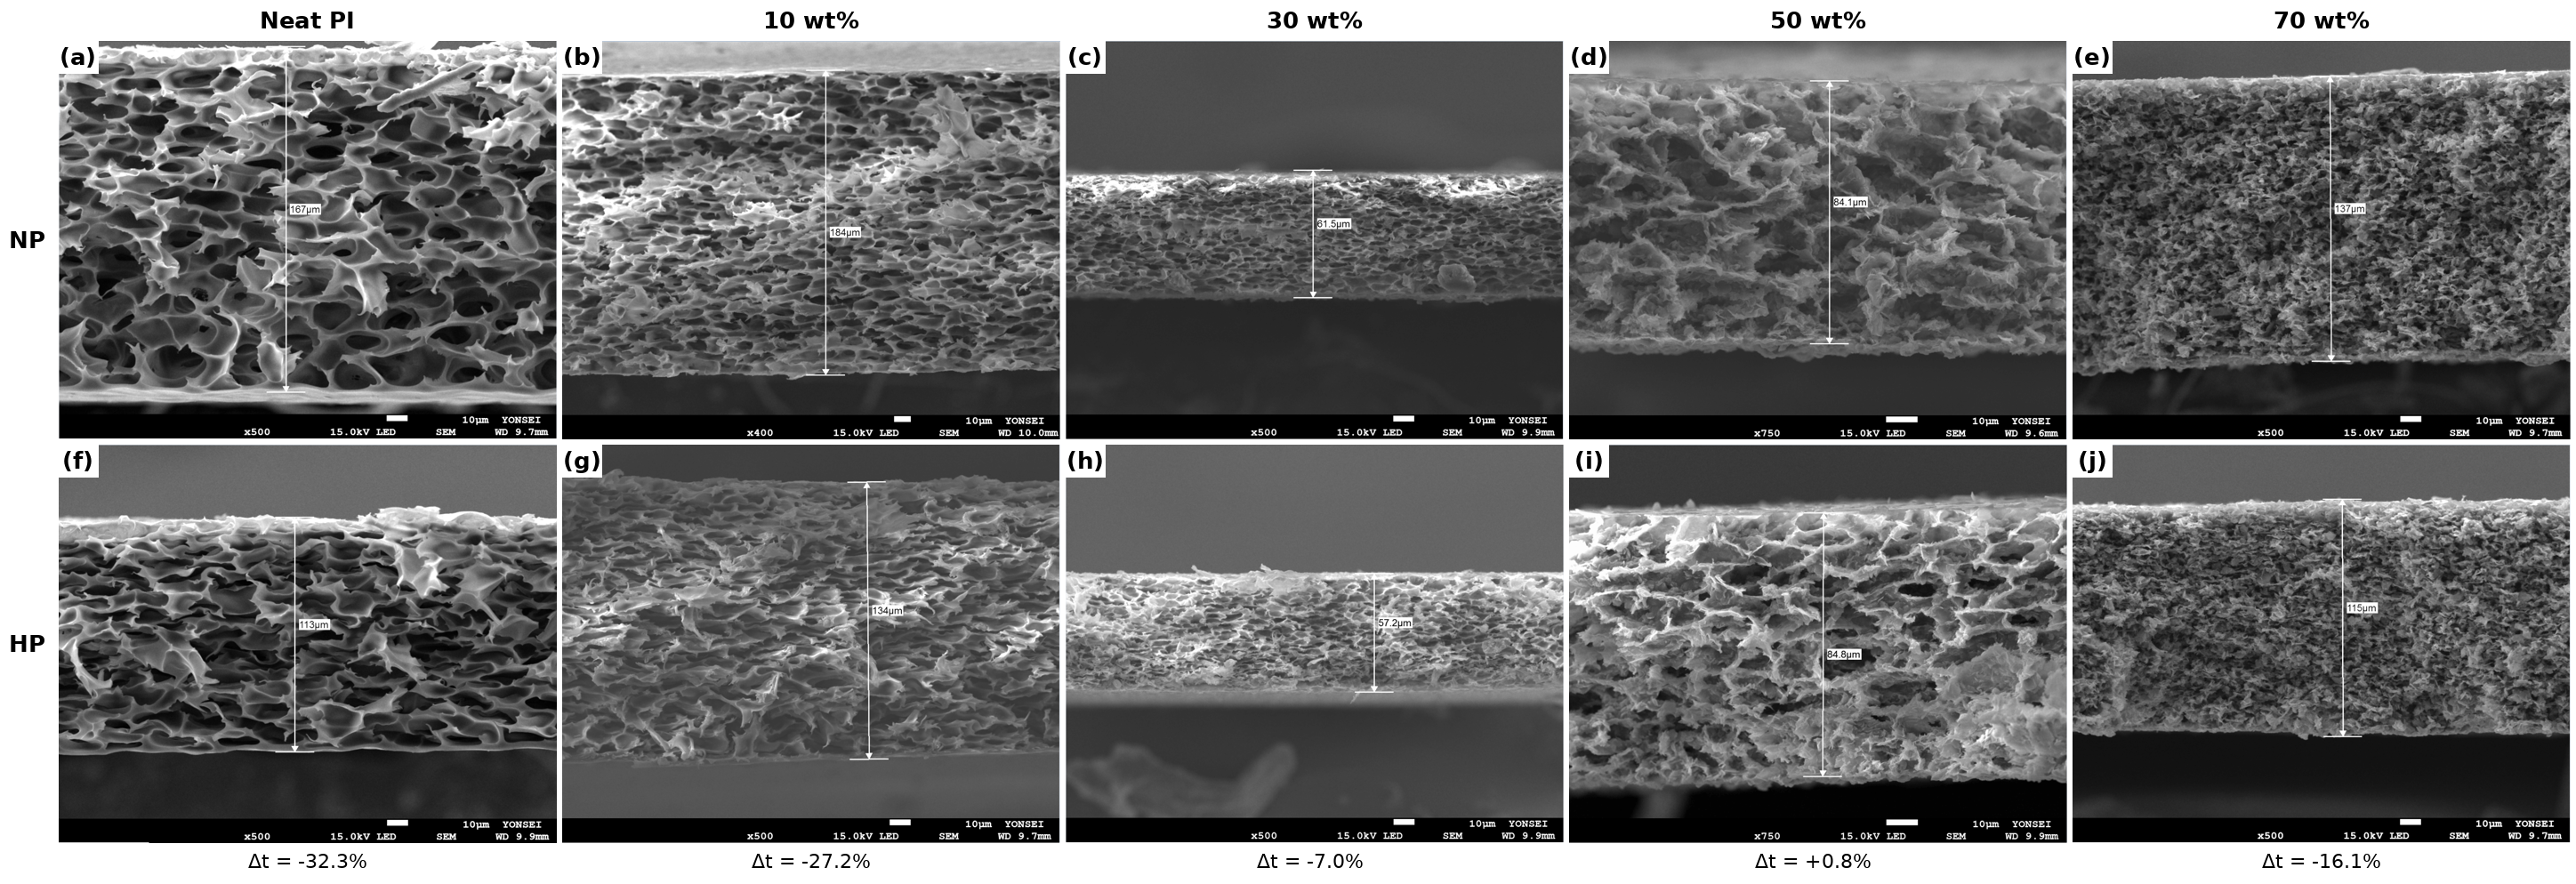
\includegraphics[width=0.99\linewidth]{Fig1.png}
\caption{Cross-sectional FE-SEM micrographs of PI/h-BN films at 0--70~wt\% h-BN in the non-pressed (a--e, top row) and hot-pressed (f--j, bottom row) states. $\Delta t$ denotes the film-thickness change upon hot-pressing. Top-view micrographs and EDS elemental analysis are provided in Figure~S7 and Table~S1.}
\label{fig:sem}
\end{figure}


Hot-pressed (HP) films are produced by applying uniaxial compressive force at elevated temperature to NP films. Hot-pressing collapses part of the open pore network, increasing bulk density and tensile strength. For most compositions, the HP open porosity is substantially lower than the NP value (43.4\% vs.\ 75.4\% for neat PI; 29.8\% vs.\ 91.4\% for 10~wt\% h-BN), whereas the 30 and 50~wt\% HP films show higher intrusion porosities than their NP counterparts (67.2\% vs.\ 48.8\% and 64.6\% vs.\ 58.1\%). Mercury intrusion probes only the open, connected pore volume. The total porosity from the bulk density, $\phi_{\mathrm{total}} = 1 - \rho/\rho_{\mathrm{solid}}$ (Table~\ref{tab:thermo}), exceeds the intrusion value for six of the seven films for which $\rho$ was measured, by up to 31 percentage points (NP 30~wt\%: 79.8\% vs.\ 48.8\%); the difference is a measure of closed porosity. Notably, $\phi_{\mathrm{total}}$ decreases from NP to HP at every composition (30~wt\%: $79.8 \to 71.6\%$; 50~wt\%: $70.6 \to 61.3\%$; 70~wt\%: $72.8 \to 72.1\%$), so the reversed NP/HP ordering of the intrusion values at 30 and 50~wt\% reflects a change in pore connectivity, in which compaction opens previously closed pores to intrusion, rather than an increase in total pore volume. Both quantities are tabulated in Table~\ref{tab:thermo}, and the choice of porosity input to Eq.~\ref{eq:step2} is discussed in Section~\ref{sec:dielectric}. SEM cross-sections (Figure~\ref{fig:sem}) confirm thickness reductions of 32.3\%, 27.2\%, and 16.1\% at 0, 10, and 70~wt\% h-BN, whereas the 30 and 50~wt\% films show near-zero thickness change ($-7.0\%$ and $+0.8\%$), consistent with the resistance of the h-BN network to compaction at these loadings. EDS elemental analysis (Table~S1) confirms that the boron content scales systematically with nominal loading (B: 8.0 to 29.3~wt\% from 10 to 70~wt\% h-BN, NP series) and is preserved upon hot-pressing, verifying composition retention through the NIPS and densification steps; the apparent B signal of 5.4~wt\% in the neat film reflects the quantification limit of EDS for light elements and is treated as background.

EDS elemental mapping confirms near-quantitative h-BN incorporation at $\geq$10~wt\% h-BN, with measured boron weight fractions within $\pm$5~wt\% (absolute) of the theoretical values. Spot-to-spot variance ($<$1~wt\% B at 70~wt\% h-BN) confirms homogeneous h-BN dispersion achieved by the sonication-assisted NIPS protocol.

\subsection{Dielectric constant}
\label{sec:dielectric}
Figure~\ref{fig:transport}a presents the measured dielectric constants and the three-phase LN predictions for all ten samples; the corresponding parity plot is given in Figure~S2. All films exhibit \eps{} far below dense PI ($\sim$3.5), confirming that NIPS-generated porosity dominates the dielectric response. NP films reach $\eps = 1.28$--1.76 (\SI{100}{\kilo\hertz}) and HP films span $\eps = 1.62$--2.18. Hot-pressing raises \eps{} by $\Delta\eps = 0.18$--0.42 at every composition through pore collapse. In the NP series \eps{} decreases monotonically with h-BN content ($1.76 \to 1.28$); because $\varepsilon_{\mathrm{BN}}$ ($\sim$6) exceeds $\varepsilon_{\mathrm{PI}}$ ($\sim$3.5) and the open porosity does not increase over this range, no mixing rule reproduces this trend (Section~S3.5), and the model predictions evaluated at each film's open porosity follow the porosity input rather than the composition (Figure~\ref{fig:transport}a).

\begin{figure}[htbp]
\centering
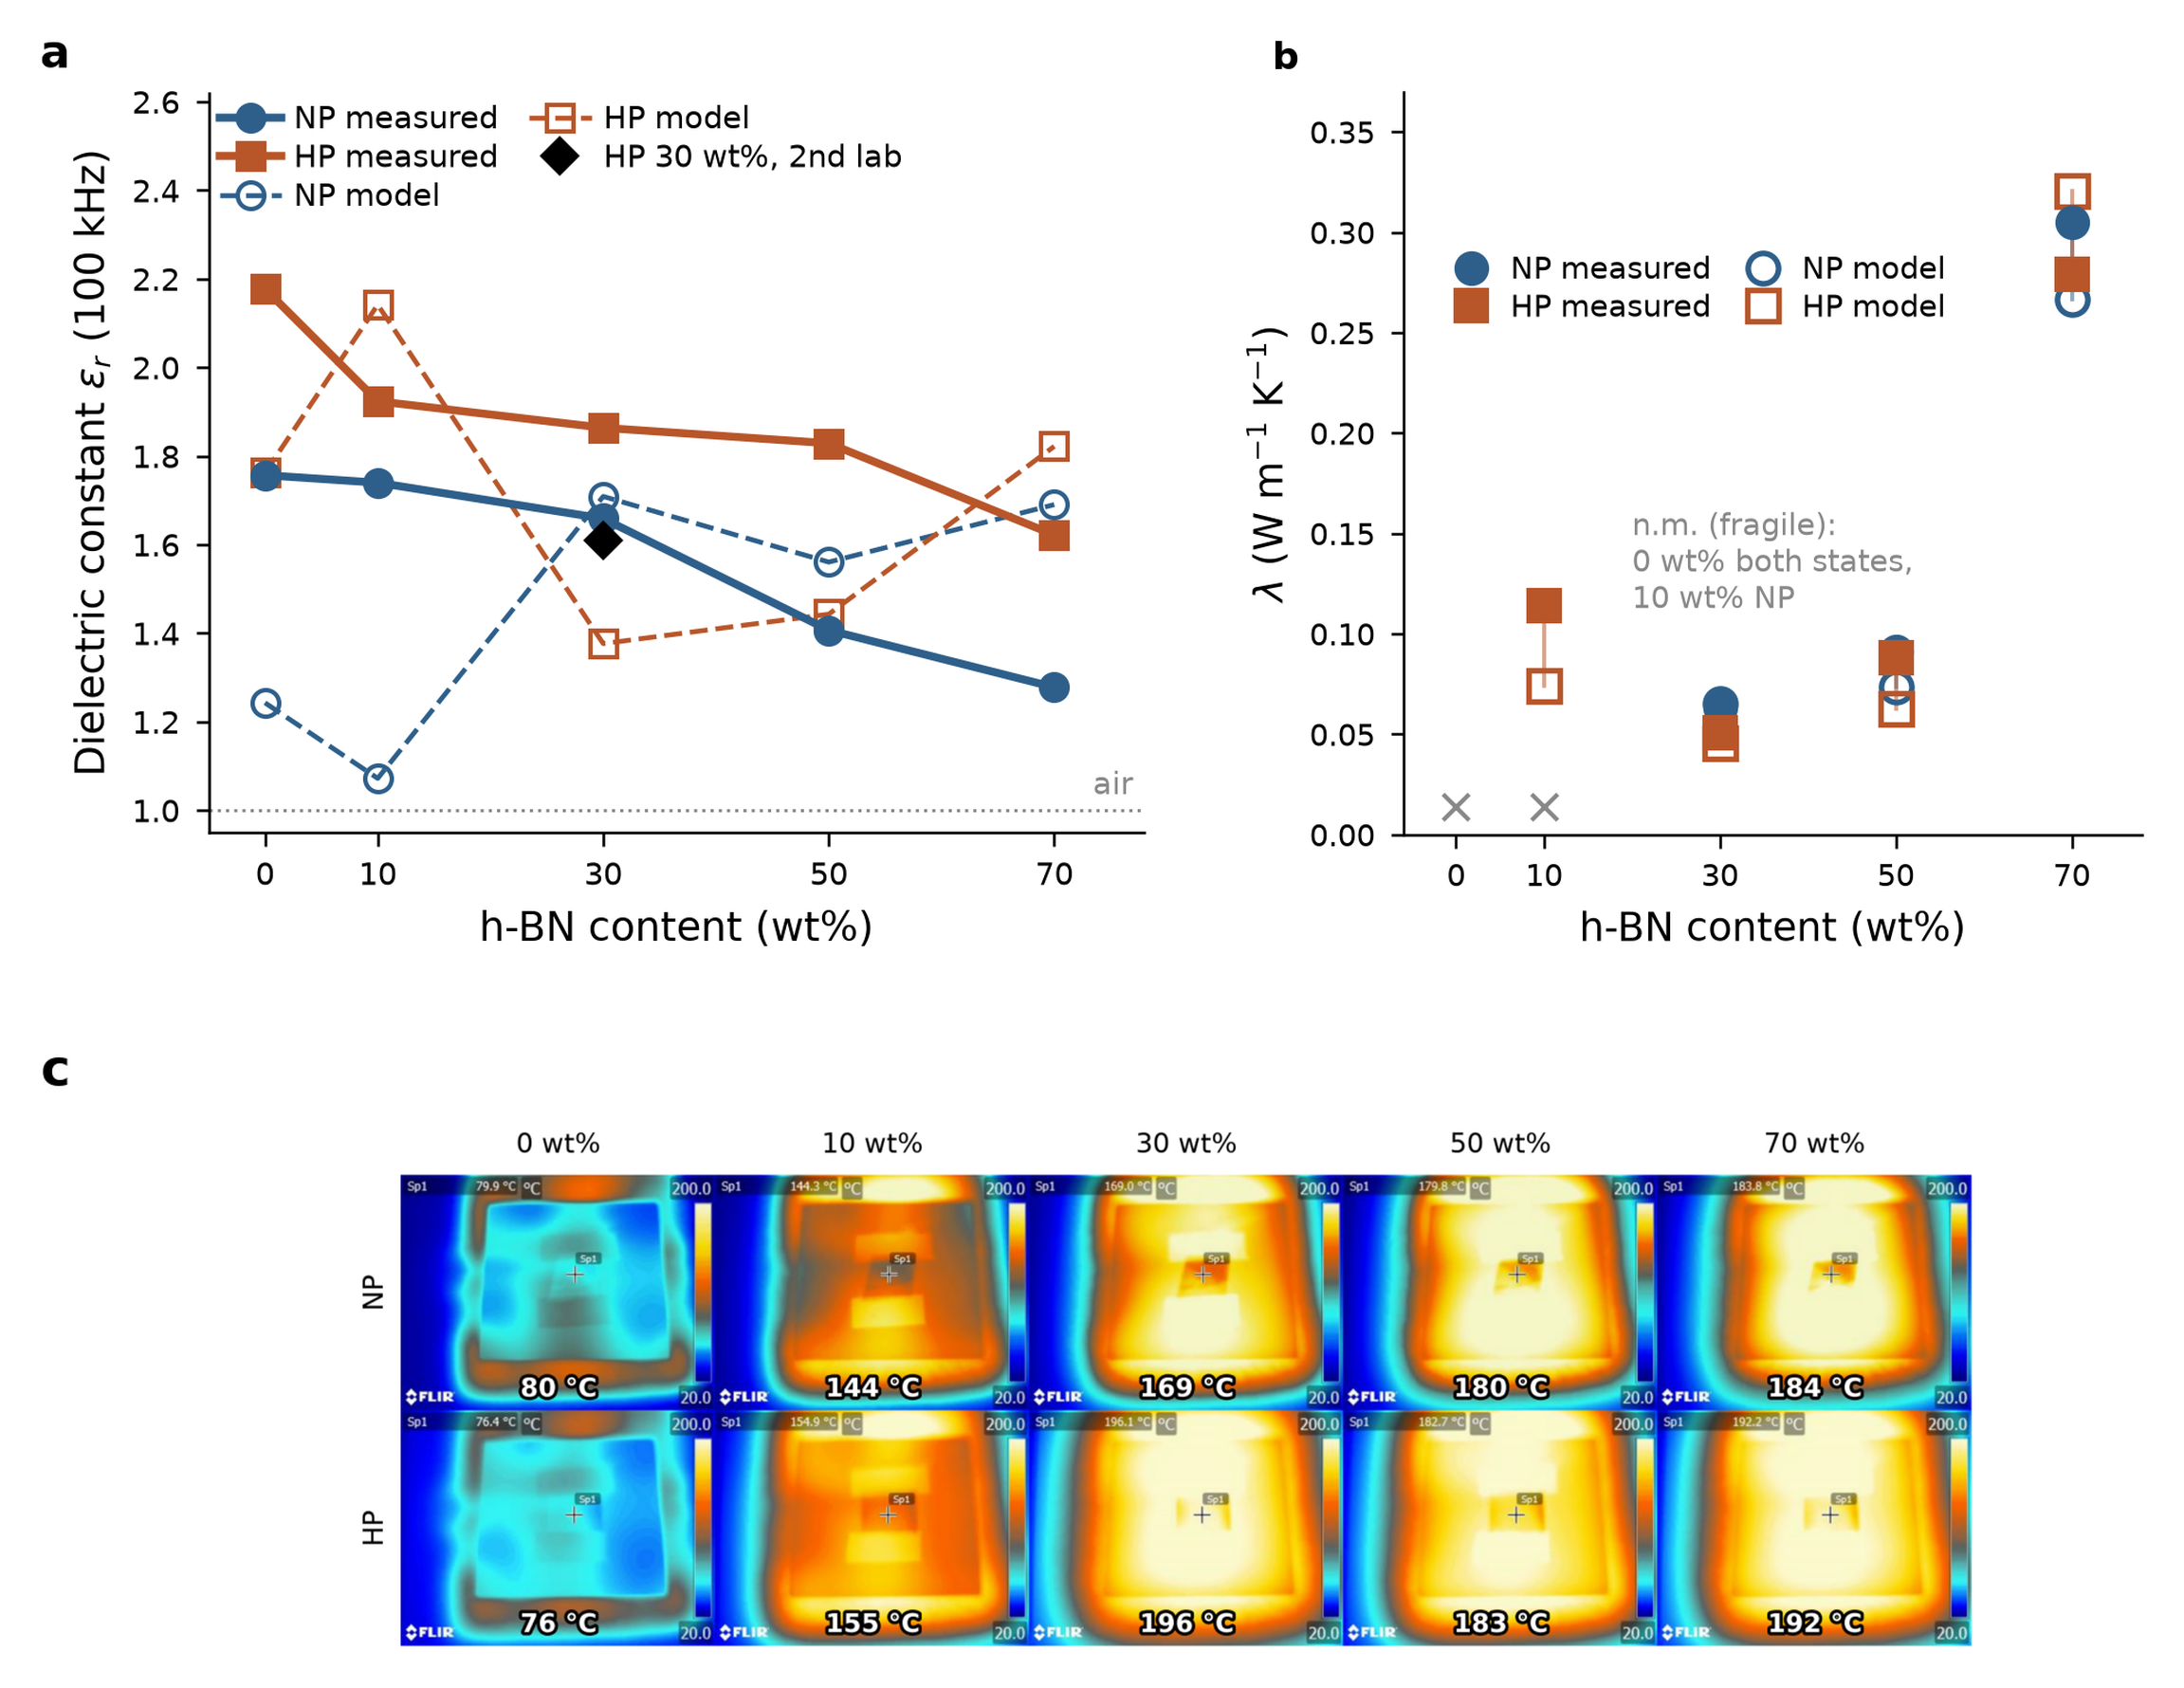
\includegraphics[width=0.98\linewidth]{Fig2.png}
\caption{Measured dielectric and thermal properties of PI/h-BN films ($n = 1$ per condition). (a) Dielectric constant at \SI{100}{\kilo\hertz} vs.\ h-BN content for NP and HP films; filled symbols, measured; open symbols joined by dashed lines, three-phase LN predictions at each film's measured open porosity; black diamond, independent measurement of the HP 30~wt\% film (KOPTRI, ASTM D150), not used in fitting. (b) Thermal conductivity vs.\ h-BN content; open symbols, single-parameter LN predictions (\lamBN{} fitted; $A = 5.5$, $\phimax = 0.60$ fixed), joined to the measured value by a tie-line; crosses mark compositions that could not be measured (film fragility). (c) Infrared thermography of all ten films on a \SI{200}{\celsius} stage after \hl{X}~min equilibration; annotated values are uncorrected radiometric spot temperatures and are comparative, not absolute. Parity plot and porosity-sensitivity curves are given in Figures~S2 and S3.}
\label{fig:transport}
\end{figure}

The LN model returns RMSE = 0.43 (NP) and 0.36 (HP), which exceeds the standard deviation of the measured \eps{} across compositions (0.19 NP, 0.18 HP); the coefficient of determination is therefore negative ($R^2 = -3.9$ NP, $-3.0$ HP; $-1.6$ for the 30--70~wt\% subset). The calibrated model does not predict \eps{} for individual films better than the data mean, and we use it accordingly: as a mechanistic description of how porosity and pore geometry enter \eps, and as a generator of design maps whose absolute levels carry an uncertainty of the order of the RMSE. Part of the residual is attributable to the porosity input itself. The fits use the open porosity as $\phi_p$ in Eq.~\ref{eq:step2}, the quantity available for all ten films; because \eps{} and \lam{} respond to the total air fraction irrespective of its connectivity, $\phi_{\mathrm{total}}$ is the physically appropriate input, but it is available only for the seven films with measured density and differs from the open porosity by up to 31 percentage points (Section~\ref{sec:morphology}). The largest residuals occur at 0, 10, and 70~wt\% in the NP series (model underprediction of 29--38\% at 0--10~wt\% and overprediction of 32\% at 70~wt\%, Table~\ref{tab:dielectric}).

Two physical mechanisms explain the systematic underprediction at low h-BN loading. First, at these compositions, the NP films exhibit extremely high porosities (75.4\% and 91.4\%, respectively). At $\phi_p > 0.75$, the sponge pore network transitions from a regime of moderate connectivity (where the mean-field $\Apore = 0.08$ provides adequate description) to a near-fully-open framework where the PI skeleton itself becomes discontinuous. In this regime, the effective dielectric constant is dominated by long-range pore connectivity and wall-thinning effects that are outside the scope of a local mean-field mixing rule. Second, at 10~wt\% h-BN with 91.4\% porosity, the h-BN volume fraction in the film is only $\phi_{\mathrm{BN,film}} = 0.006$, so the dielectric response should approach that of a PI foam. For the limiting inverted topology (isolated PI inclusions in air), the dilute Maxwell--Garnett estimate $\eps \approx 1 + 3\phi_s(\varepsilon_{\mathrm{PI}}-1)/(\varepsilon_{\mathrm{PI}}+2)$ at solid fraction $\phi_s \approx 0.087$ gives $\eps \approx 1.12$, also far below the measured 1.74. The NIPS film at this extreme porosity likely exhibits a partially inverted topology that neither the Maxwell--Garnett nor the Lewis--Nielsen mean-field picture captures: the measured value indicates that the real PI skeleton remains substantially more connected than either idealized topology assumes. These limitations are inherent to mean-field approaches and do not affect conclusions at compositions with moderate porosity (30--70~wt\% h-BN), where the RMSE restricted to the NP films of this range is 0.25.

An independent measurement of the HP 30~wt\% film at KOPTRI (ASTM D150) gives $\eps = 1.610$, compared with 1.864 in-house ($-13.6\%$ inter-laboratory deviation) and a model prediction of 1.376 at the open porosity of 67.2\% (Figure~\ref{fig:transport}a, black diamond; Table~\ref{tab:dielectric}). The three values disagree pairwise at the 14\% level. The inter-laboratory difference is an estimate of the reproducibility of \eps{} measurements on porous films with contact electrodes: an air gap between a rough porous surface and the electrode acts as a series capacitance that lowers the apparent \eps{} by an amount that depends on surface texture, and therefore on composition and processing state. This effect is a plausible experimental contributor to the negative $R^2$ and to the composition trend of the NP series noted above, and re-measurement with sputtered or painted electrodes would resolve it. The model residual at 30~wt\% HP ($-26\%$) exceeds the inter-laboratory spread and is therefore a model limitation rather than a measurement artefact.

\begin{table}[htbp]
\centering
\caption{Experimental vs.\ predicted dielectric constants (three-phase Lewis--Nielsen model). KOPTRI: independent inter-laboratory measurement of the HP 30~wt\% film (ASTM D150; not used in fitting).}
\label{tab:dielectric}
\small
\begin{tabular}{@{}cccccccc@{}}
\toprule
h-BN & $\varepsilon_{r,\mathrm{NP}}$ & $\varepsilon_{r,\mathrm{NP}}$ & $\Delta$ & $\varepsilon_{r,\mathrm{HP}}$ & $\varepsilon_{r,\mathrm{HP}}$ & $\Delta$ & KOPTRI \\
(wt\%) & (Exp.) & (LN) & (\%) & (Exp.) & (LN) & (\%) & (HP) \\
\midrule
0  & 1.757 & 1.242 & $-29.3$ & 2.178 & 1.760 & $-19.2$ & --- \\
10 & 1.740 & 1.073 & $-38.4$ & 1.924 & 2.139 & $+11.2$ & --- \\
30 & 1.659 & 1.707 & $+2.9$  & 1.864 & 1.376 & $-26.2$ & 1.610$^{*}$ \\
50 & 1.407 & 1.560 & $+10.8$ & 1.829 & 1.442 & $-21.2$ & --- \\
70 & 1.278 & 1.689 & $+32.1$ & 1.622 & 1.819 & $+12.2$ & --- \\
\bottomrule
\end{tabular}\\[3pt]
\parbox{0.95\linewidth}{\footnotesize $\Delta = (\varepsilon_{r,\mathrm{LN}} - \varepsilon_{r,\mathrm{Exp}})/\varepsilon_{r,\mathrm{Exp}} \times 100\%$. LN predictions are evaluated at each film's open porosity. $^{*}$Inter-laboratory deviation from the in-house HP value (1.864) is $-13.6\%$; the model prediction at the open porosity of 67.2\% is 1.376 (Section~\ref{sec:dielectric}).}
\end{table}

\subsection{Thermal conductivity}
\label{sec:thermal}
Figure~\ref{fig:transport}b shows thermal conductivity results, and Table~\ref{tab:thermo} lists the underlying laser-flash data (bulk density, specific heat, and thermal diffusivity) together with the open and total porosities. Measurements were unavailable for the neat films in both states and for NP 10~wt\% due to film fragility at these high-porosity compositions (up to 91.4\%), leaving seven measured data points. For all available data, the single-parameter LN calibration reproduces the trends well ($\mathrm{RMSE}_{\mathrm{NP}} = 0.027$, $\mathrm{RMSE}_{\mathrm{HP}} = \SI{0.030}{\watt\per\meter\per\kelvin}$): near-constant \lam{} at 30--50~wt\% h-BN and a sharp increase at 70~wt\%. Within the model, the 70~wt\% upturn arises from the packing-interaction term $\psi$ in Eq.~\ref{eq:step1}: at $\phiBN = 0.591 \approx 0.99\,\phimax$, the composite approaches the maximum platelet packing, which is the Lewis--Nielsen representation of imminent particle--particle contact (percolation).

\begin{table}[htbp]
\centering
\caption{Porosity and thermophysical data underlying the thermal-conductivity determination ($\lam = \alpha\rho C_p$; laser flash at \SI{25}{\celsius}). $\phi_{\mathrm{open}}$: mercury intrusion; $\phi_{\mathrm{total}} = 1-\rho/\rho_{\mathrm{solid}}$ with $\rho_{\mathrm{PI}} = 1.42$ and $\rho_{\mathrm{BN}} = \SI{2.29}{\gram\per\cubic\centi\meter}$.}
\label{tab:thermo}
\footnotesize
\begin{tabular}{@{}cccccccc@{}}
\toprule
h-BN & State & $\phi_{\mathrm{open}}$ & $\phi_{\mathrm{total}}$ & $\rho$ & $C_p$ & $\alpha$ & \lam \\
(wt\%) & & (\%) & (\%) & (\si{\gram\per\cubic\centi\meter}) & (\si{\joule\per\gram\per\kelvin}) & (\si{\milli\meter\squared\per\second}) & (\si{\watt\per\meter\per\kelvin}) \\
\midrule
0  & NP & 75.4 & ---  & ---   & ---   & ---   & --- \\
0  & HP & 43.4 & ---  & ---   & ---   & ---   & --- \\
10 & NP & 91.4 & ---  & ---   & ---   & ---   & --- \\
10 & HP & 29.8 & 40.4 & 0.879 & 0.903 & 0.143 & 0.114 \\
30 & NP & 48.8 & 79.8 & 0.323 & 0.853 & 0.230 & 0.063 \\
30 & HP & 67.2 & 71.6 & 0.455 & 0.863 & 0.131 & 0.051 \\
50 & NP & 58.1 & 70.6 & 0.515 & 0.875 & 0.202 & 0.091 \\
50 & HP & 64.6 & 61.3 & 0.678 & 0.885 & 0.147 & 0.088 \\
70 & NP & 54.2 & 72.8 & 0.526 & 0.838 & 0.693 & 0.305 \\
70 & HP & 48.8 & 72.1 & 0.539 & 0.846 & 0.613 & 0.279 \\
\bottomrule
\end{tabular}\\[3pt]
\parbox{0.95\linewidth}{\footnotesize Neat PI (both states) and NP 10~wt\% could not be measured by laser flash (film fragility), and $\rho$ was not determined for these films. The LN fits use $\phi_{\mathrm{open}}$ as the porosity input (Section~\ref{sec:dielectric}).}
\end{table}


The fitted $\lamBN = \SI{6.81}{\watt\per\meter\per\kelvin}$ lies well below the through-plane conductivity of bulk h-BN ($\sim$\hl{value}~\si{\watt\per\meter\per\kelvin}~\cite{guerra2019thermal}), which we attribute primarily to Kapitza thermal interface resistance at the h-BN--PI interface. At \SI{70}{\nm} particle diameter, the surface-area-to-volume ratio is approximately \SI{30}{\meter\squared\per\gram}, causing interfacial phonon scattering to limit heat transfer through individual particles; this is consistent in order of magnitude with molecular-dynamics-based interfacial conductance estimates for h-BN--polymer interfaces ($G \sim 10$--\SI{100}{\mega\watt\per\meter\squared\per\kelvin}), which at \SI{70}{\nm} correspond to effective particle conductivities of order 1--\SI{7}{\watt\per\meter\per\kelvin}~\cite{gu2021breaking}. Two residual features carry physical information, with the caveat that both are comparable to the $\sim$10\% propagated uncertainty in \lam{} (Section~\ref{sec:char}). First, the NP 70~wt\% film exceeds the model prediction (0.305 vs.\ \SI{0.263}{\watt\per\meter\per\kelvin}, $+16\%$), consistent with incipient h-BN--h-BN contact beyond the mean-field description. Second, hot-pressing at 70~wt\% reduces \lam{} ($0.305 \to \SI{0.279}{\watt\per\meter\per\kelvin}$) while the open porosity decreases ($54.2 \to 48.8\%$) and the total porosity is nearly unchanged ($72.8 \to 72.1\%$), opposite to the model trend (predicted increase to 0.315): this indicates that compaction partially disrupts the h-BN--h-BN contact network formed during NIPS, sacrificing percolative pathways even as the solid fraction increases. Porosity sensitivity at fixed composition (Figure~S3) shows that both properties remain strongly porosity-coupled at 50~wt\%: over the experimentally accessible 30--65\% porosity range, \eps{} spans 1.43--2.31 while \lam{} spans 0.06--\SI{0.16}{\watt\per\meter\per\kelvin}.

\subsection{Tensile strength and coefficient of thermal expansion}
\label{sec:mechanical}
Figure~\ref{fig:mech} presents tensile strength and CTE results. Hot-pressing consistently improves tensile strength by 19--95\% (Table~\ref{tab:mechanical}), consistent with pore collapse under compressive load. The NP tensile strength is non-monotonic, with a local maximum at 30~wt\% (\SI{25.4}{\mega\pascal}) and minima at 10~wt\% (\SI{14.9}{\mega\pascal}) and 50~wt\% (\SI{12.5}{\mega\pascal}), and correlates inversely with the porosities at 10~wt\% (91.4\%) and 50~wt\% (58.1\%). The LN + Gibson--Ashby model reproduces this trend qualitatively.

\begin{figure}[htbp]
\centering
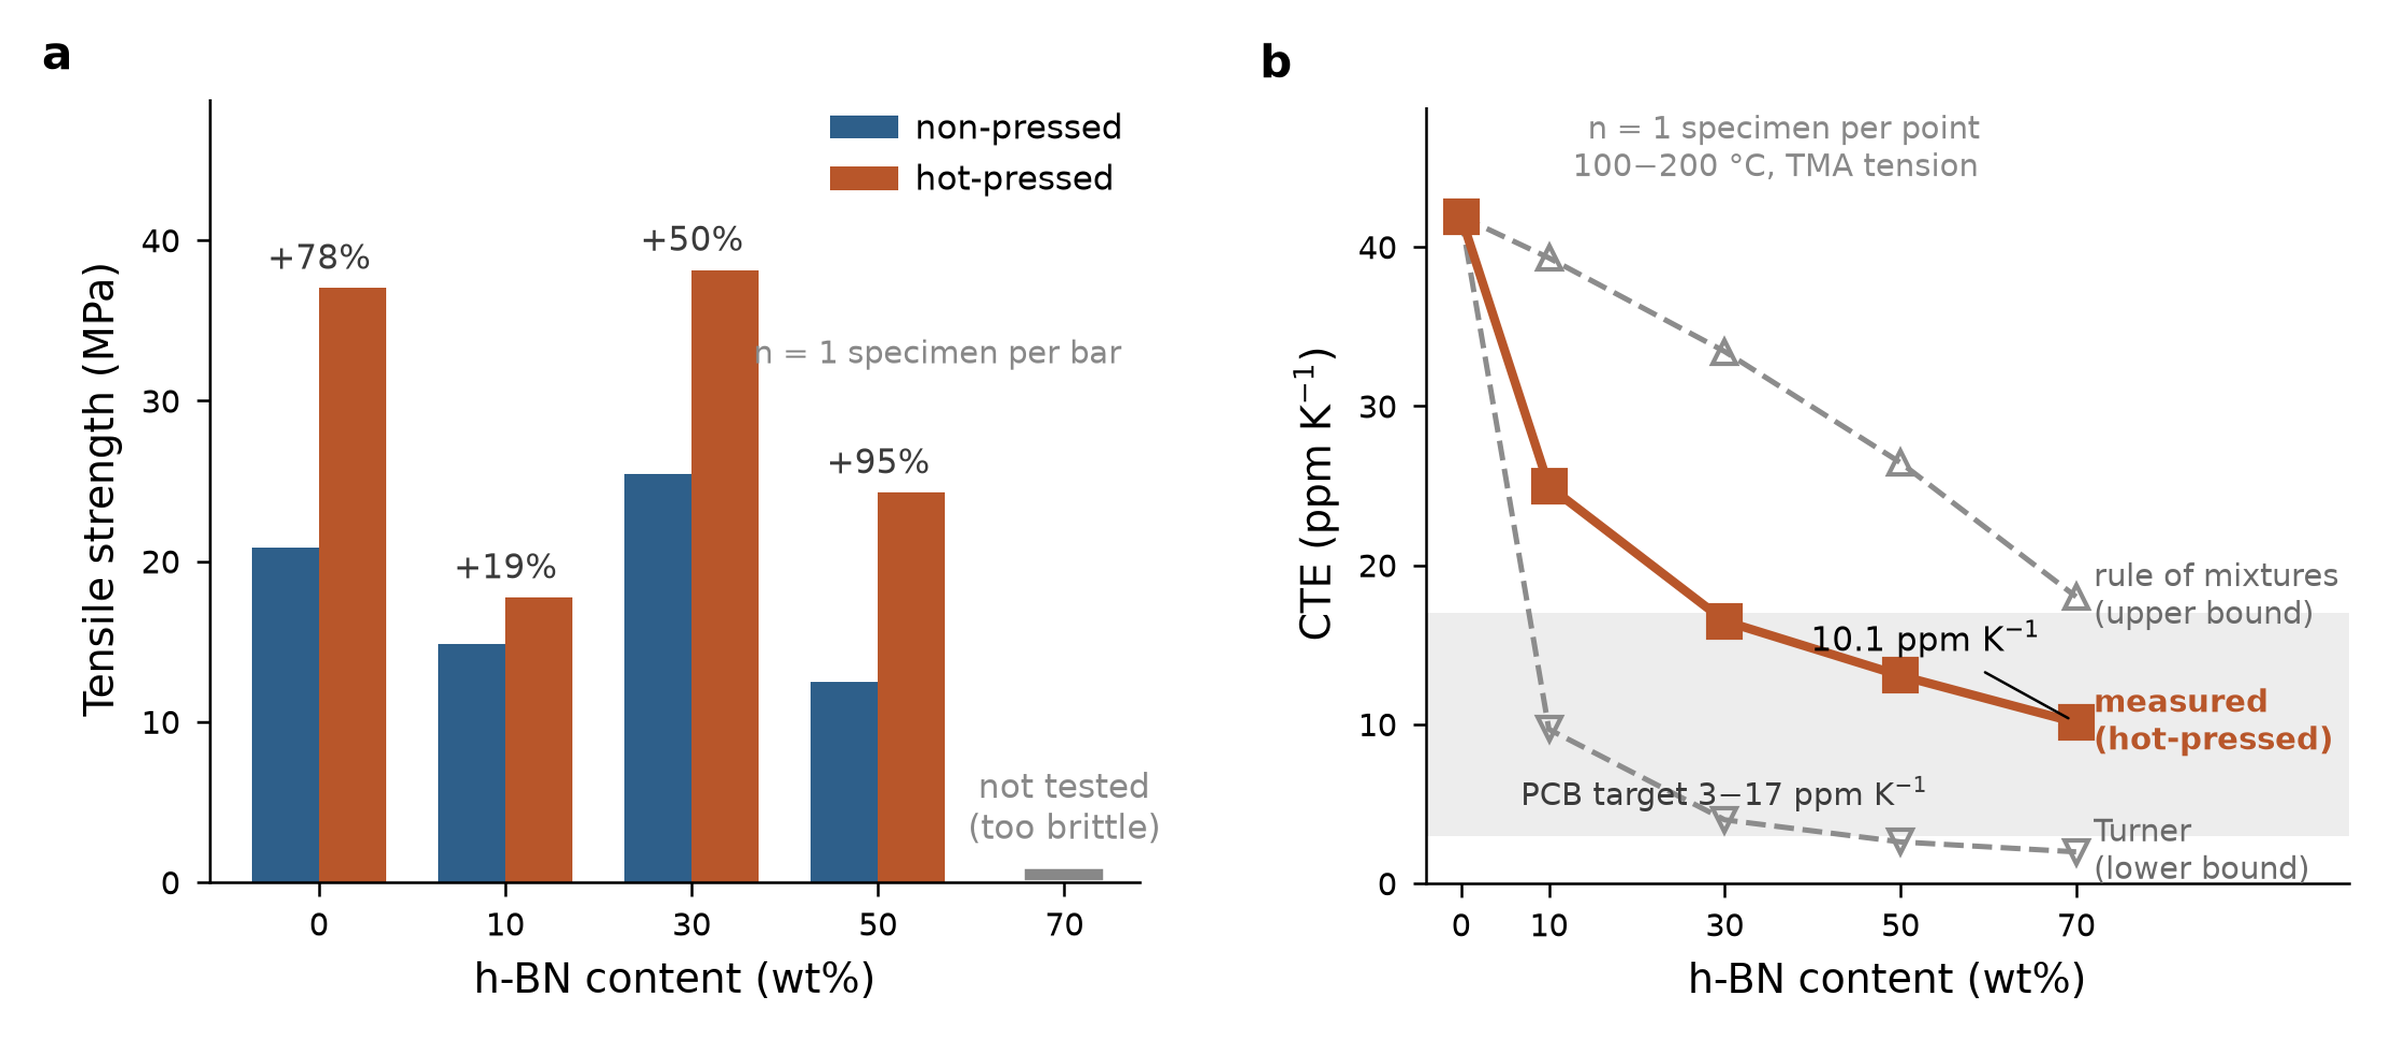
\includegraphics[width=0.98\linewidth]{Fig3.png}
\caption{Mechanical and thermal-expansion behavior of PI/h-BN films. (a) Tensile strength vs.\ h-BN content for NP and HP films ($n=1$ specimen per bar). Percentage values indicate the NP$\to$HP change at each composition; the 70~wt\% slot carries a baseline stub because those films were too brittle to test, not because the strength is zero. (b) CTE vs.\ h-BN content for HP films ($n=1$ per point; TMA, tension mode, 100--\SI{200}{\celsius}): measured values against the Turner lower bound and the rule-of-mixtures (ROM) upper bound, both computed with $\alpha_{\mathrm{PI}} = \SI{41.92}{\ppm\per\kelvin}$ (measured). The PCB substrate target zone (3--\SI{17}{\ppm\per\kelvin}) is shaded. The measured CTE lies between the two bounds because the discontinuous load-path geometry of the porous sponge gives only partial elastic constraint (Section~\ref{sec:cte}).}
\label{fig:mech}
\end{figure}

For CTE (Figure~\ref{fig:mech}b), the Turner model (using $\alpha_{\mathrm{PI}} = \SI{41.92}{\ppm\per\kelvin}$ as measured on the neat PI HP film) correctly predicts the neat-film value but substantially underpredicts CTE at all h-BN loadings ($-61$ to $-80\%$). The ROM overestimates because it neglects elastic constraint entirely. The experimental CTE values ($24.96 \to \SI{10.11}{\ppm\per\kelvin}$ from $10 \to 70$~wt\%) lie between the two model bounds, physically consistent with partial elastic constraint in a porous sponge where h-BN platelets are embedded within discontinuous PI ligaments rather than a macroscopically continuous dense matrix. This porous-architecture effect is a limitation of applying dense-composite CTE models to sponge materials and an opportunity for future model development incorporating open-cell foam mechanics. The measured CTE of \SI{10.1}{\ppm\per\kelvin} at 70~wt\% h-BN (HP) lies within the PCB substrate compatibility window (3--\SI{17}{\ppm\per\kelvin}). \hl{CTE was measured on the HP films only; the NP films at $\geq$50~wt\% were too fragile for TMA clamping.}

\begin{table}[htbp]
\centering
\caption{Tensile strength and CTE data for PI/h-BN composite films.}
\label{tab:mechanical}
\footnotesize
\begin{tabular}{@{}ccccccc@{}}
\toprule
h-BN & NP strength & HP strength & NP$\to$HP & HP CTE & Turner & ROM \\
(wt\%) & (\si{\mega\pascal}) & (\si{\mega\pascal}) & (\%) & (\si{\ppm\per\kelvin}) & (\si{\ppm\per\kelvin}) & (\si{\ppm\per\kelvin}) \\
\midrule
0  & 20.85 & 37.02 & $+77.6$ & 41.92 & 41.92 & 41.92 \\
10 & 14.86 & 17.74 & $+19.4$ & 24.96 & 9.69  & 39.31 \\
30 & 25.43 & 38.15 & $+50.0$ & 16.49 & 4.00  & 33.43 \\
50 & 12.47 & 24.28 & $+94.7$ & 13.06 & 2.61  & 26.45 \\
70 & ---$^{*}$ & ---$^{*}$ & --- & 10.11 & 1.98 & 18.02 \\
\bottomrule
\end{tabular}\\[3pt]
\parbox{0.95\linewidth}{\footnotesize $^{*}$Not tested (film brittleness at 70~wt\% h-BN). Turner and ROM use $\alpha_{\mathrm{PI}} = \SI{41.92}{\ppm\per\kelvin}$ (measured neat porous PI, HP), $E_{\mathrm{PI}} = \SI{3.5}{\giga\pascal}$, $E_{\mathrm{BN}} = \SI{200}{\giga\pascal}$, $\alpha_{\mathrm{BN}} = \SI{1.5}{\ppm\per\kelvin}$, solid-phase volume fractions.}
\end{table}

\subsection{Design maps for simultaneous property optimization}
\label{sec:designmaps}
Figure~\ref{fig:design}a,b presents model-generated design maps of \eps{} and \lam{} spanning the full composition space (h-BN content 0--70~wt\%; porosity 0--95\%), with experimental NP and HP states overlaid and arrows indicating the NP$\to$HP processing trajectory at each composition.

\begin{figure}[htbp]
\centering
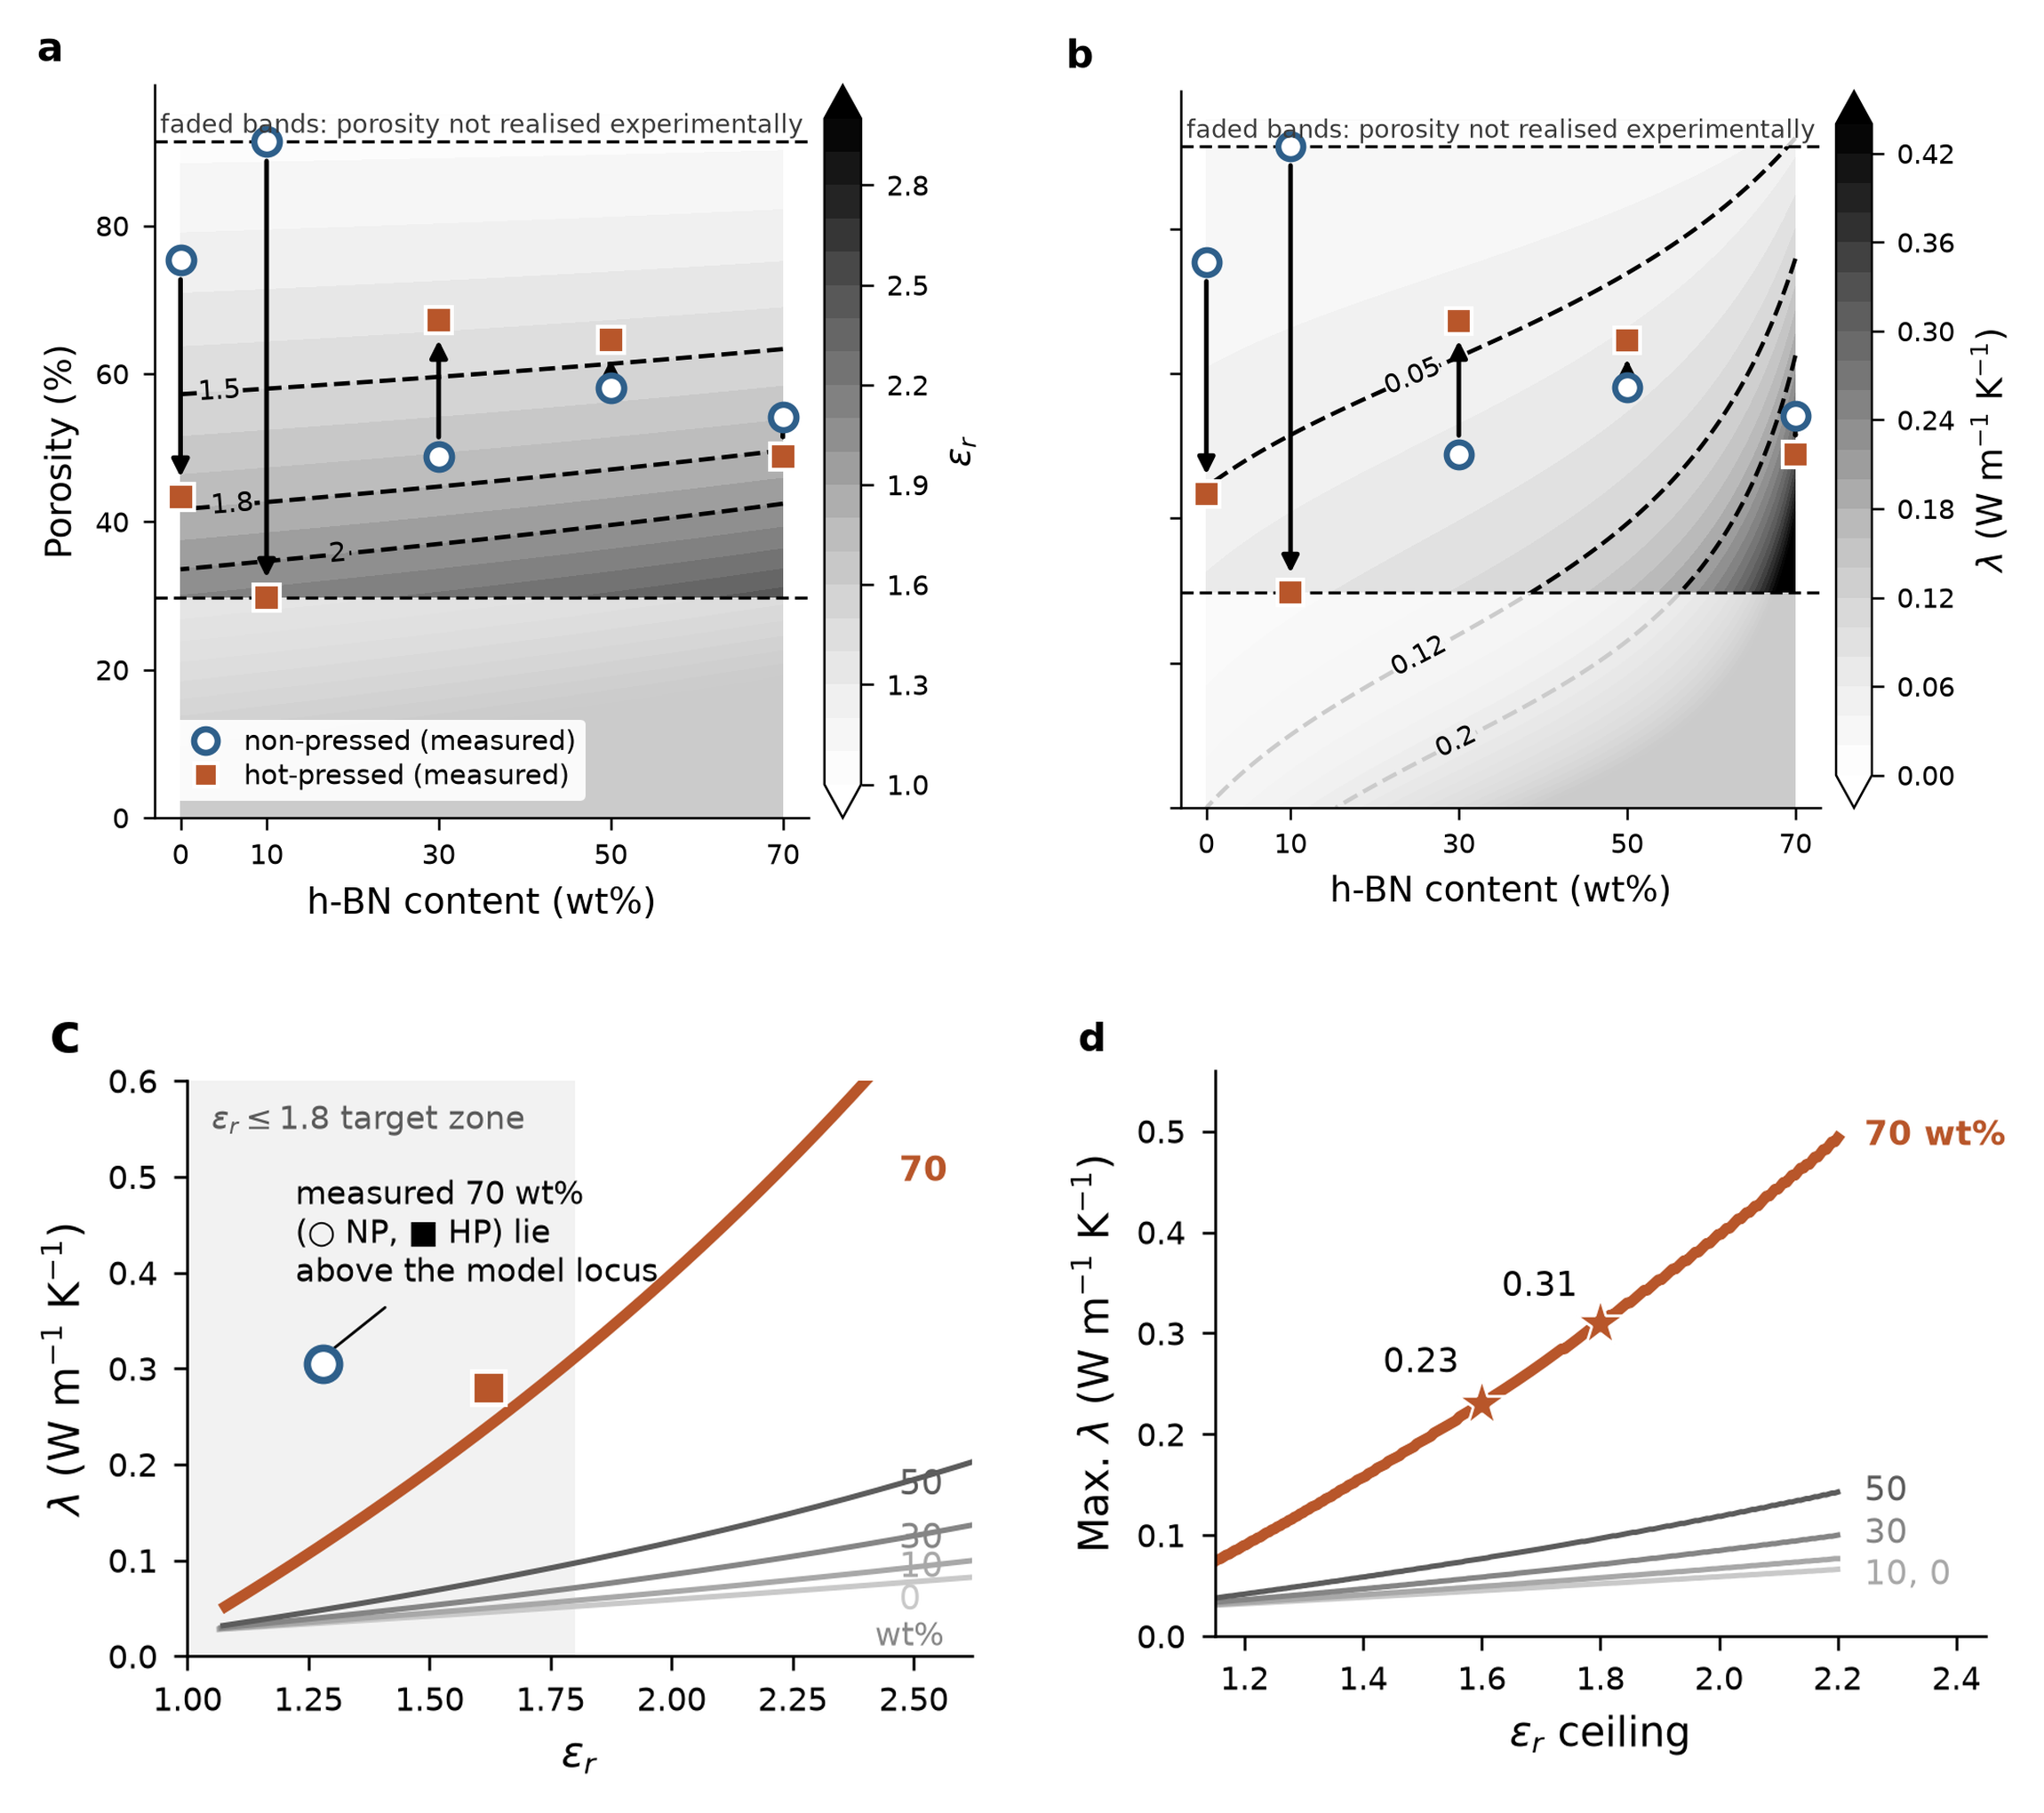
\includegraphics[width=0.98\linewidth]{Fig4.png}
\caption{Model-guided design (three-phase LN model, calibration of Table~\ref{tab:params}). (a, b) Design maps of \eps{} and \lam{} vs.\ h-BN content and porosity; measured NP (open circles) and HP (filled squares) states overlaid, arrows indicating the NP$\to$HP trajectory; faded bands above 91\% and below 30\% porosity lie outside the range realized by any film. (c) \eps--\lam{} loci for each loading with porosity swept along each curve; the measured 70~wt\% films lie above their own locus. (d) Maximum \lam{} attainable under a given \eps{} ceiling with porosity optimized at each point; stars mark the $\eps \le 1.6$ and $\eps \le 1.8$ operating points at 70~wt\%. The absolute levels of panels (a)--(d) inherit the dielectric uncertainty quantified in Section~\ref{sec:dielectric}. Feasible-window and porosity-optimum panels are given in Figures~S4 and S5.}
\label{fig:design}
\end{figure}

Three actionable design principles emerge. First, achieving $\eps < 1.5$ requires porosity above $\sim$57\% at low h-BN loading, rising to $\sim$63\% at 70~wt\%, a range accessible to NIPS in both NP and moderately pressed states. Second, \lam{} is strongly loading-gated: $\lam > \SI{0.20}{\watt\per\meter\per\kelvin}$ is unreachable below $\sim$55~wt\% h-BN at any practical porosity, requires porosity below $\sim$35\% at 60~wt\%, but is available up to $\sim$62\% porosity at 70~wt\%; the packing-limit amplification at high loading relaxes the porosity constraint. Third, the NP$\to$HP trajectories show that hot-pressing traverses the maps nearly vertically (porosity is the processing variable), so composition must be selected first and porosity tuned second; at 70~wt\%, both the NP and HP states already lie in the simultaneously favorable region.

\subsection{Shape-factor sensitivity}
\label{sec:shapefactor}
Figure~S1 systematically examines the sensitivity of LN predictions to the h-BN shape factor $A$ for values 0.3--6.0, corresponding to geometries from needle-like rods to highly aligned platelets.

For the dielectric model (Figure~S1a), all $A$ curves are nearly indistinguishable, confirming that \eps{} is dominated by the step~2 pore term (Eq.~\ref{eq:step2}), not by \ABN. In porous NIPS films, h-BN particle geometry has little influence on dielectric performance; only porosity level and pore architecture (\Apore) matter. This justifies treating the fitted dielectric \ABN{} as weakly determined (Table~\ref{tab:params}) and confirms that the RMSE values in Table~\ref{tab:dielectric} reflect mean-field model limitations rather than parameter uncertainty.

For the thermal model (Figure~S1b), sensitivity to $A$ is higher above 30~wt\% h-BN, which is precisely why $A$ was fixed at its literature platelet value rather than fitted (Section~\ref{sec:paramest}). At the NP mean porosity (65.6\%), all $A = 0.3$--6.0 curves remain below the experimental NP 70~wt\% value (0.16--0.18 vs.\ \SI{0.305}{\watt\per\meter\per\kelvin}), reinforcing that the 70~wt\% enhancement is driven by the proximity to maximum packing and incipient particle contact, not by any plausible choice of single-particle shape factor. In the practically important 30--50~wt\% range, the $A$ curves converge within $\pm$\SI{0.02}{\watt\per\meter\per\kelvin}, and the mean-field LN model is adequate.

\subsection{Property trade-offs and design guidance}
\label{sec:ashby}
For each h-BN loading, the calibrated LN model traces a continuous locus in \eps--\lam{} space as porosity is swept (Figure~\ref{fig:design}c); the 70~wt\% HP state already lies within the target zone ($\eps = 1.62$, $\lam = \SI{0.28}{\watt\per\meter\per\kelvin}$).

Three design insights emerge. First, along any fixed-composition locus, reducing porosity raises both \eps{} and \lam; the two properties are coupled through the same structural variable and cannot be tuned independently by porosity control alone; every porosity choice is a position on a trade-off curve. Second, increasing h-BN loading shifts the entire locus toward higher \lam{} at any given \eps, making composition the primary lever for thermal performance at constant dielectric specification. Third, the 70~wt\% locus passes through the most favorable region: experimentally, the NP film at 54.2\% open porosity ($\eps = 1.28$, $\lam = \SI{0.31}{\watt\per\meter\per\kelvin}$) meets all three target levels defined below, and the HP film at 48.8\% ($\eps = 1.62$, $\lam = \SI{0.28}{\watt\per\meter\per\kelvin}$) meets the Basic and Advanced levels.

\subsection{Model-guided design: performance limits and processing prescriptions}
\label{sec:optimization}
The calibrated model can be interrogated across the full (h-BN loading, porosity) space to identify performance limits and the processing conditions required to reach a given specification. Figure~\ref{fig:design}c,d presents this analysis; the absolute levels of the model surfaces inherit the dielectric uncertainty quantified in Section~\ref{sec:dielectric}.

The feasible processing window, defined as the porosity range that simultaneously satisfies each of three progressively demanding specifications, Basic ($\eps < 2.0$, $\lam > \SI{0.05}{\watt\per\meter\per\kelvin}$), Advanced ($\eps < 1.8$, $\lam > \SI{0.08}{\watt\per\meter\per\kelvin}$), and Future ($\eps < 1.6$, $\lam > \SI{0.12}{\watt\per\meter\per\kelvin}$), is shown in Figure~S4. The Basic window is open across the entire composition range (even neat porous PI qualifies at $\sim$34--44\% porosity, since $\lam_{\mathrm{PI}} = \SI{0.12}{\watt\per\meter\per\kelvin}$ exceeds the Basic threshold at moderate porosity); the Advanced window opens at $\geq$40~wt\% h-BN; and the Future window opens only at $\geq$64~wt\% h-BN, spanning 58--76\% porosity at 70~wt\%. Experimentally, the 70~wt\% NP film ($\eps = 1.28$, $\lam = \SI{0.31}{\watt\per\meter\per\kelvin}$) satisfies the Future specification outright, and the 70~wt\% HP film satisfies the Advanced specification; the model is conservative for \eps{} at this composition (predicting 1.69 vs.\ the measured 1.28), so the experimental films outperform the model envelope and the prescribed windows should be read as sufficient, not necessary, conditions. Figure~\ref{fig:design}c shows the \eps--\lam{} trade-off loci for all loadings together with the Pareto frontier computed over the full (loading, porosity) grid: the frontier coincides with the 70~wt\% locus over the accessible range. Because the dielectric residuals exceed the spread of the data (Section~\ref{sec:dielectric}) and the measured 70~wt\% films depart from the predicted locus ($\eps = 1.28$ measured vs.\ 1.69 predicted, NP), we read this as model-level consistency with the experimental finding that 70~wt\% is the most favorable composition tested, not as a validated frontier of the material system beyond the measured range. Figure~\ref{fig:design}d answers the engineering question `what is the maximum \lam{} achievable at a given \eps{} ceiling?': at 70~wt\%, the model envelope reaches $\lam = \SI{0.23}{\watt\per\meter\per\kelvin}$ at $\eps \leq 1.6$ (porosity 58\%), \SI{0.31}{\watt\per\meter\per\kelvin} at $\eps \leq 1.8$ (porosity 50\%), and \SI{0.39}{\watt\per\meter\per\kelvin} at $\eps \leq 2.0$ (porosity 42\%). The experimental 70~wt\% points (NP: 0.305; HP: \SI{0.279}{\watt\per\meter\per\kelvin}) lie on or slightly above the $\eps \leq 1.8$ envelope, consistent with the optimization surface in the experimentally probed region.

The optimization surface condenses into simple engineering prescriptions. The porosity that maximizes \lam{} under a fixed \eps{} ceiling is nearly independent of composition (42--50\% for $\eps \leq 1.8$ and 52--58\% for $\eps \leq 1.6$, Figure~S5), so the porosity target is set almost entirely by the dielectric ceiling, while the achievable \lam{} at that porosity is set by the h-BN loading. In terms of specific specifications, achieving $\eps < 1.7$ with $\lam > \SI{100}{\milli\watt\per\meter\per\kelvin}$ requires $\geq$60~wt\% h-BN (porosity 53--54\%); $\eps < 1.6$ with $\lam > \SI{120}{\milli\watt\per\meter\per\kelvin}$ requires 70~wt\% at 58\% porosity; and the most demanding specification ($\eps < 1.5$, $\lam > \SI{150}{\milli\watt\per\meter\per\kelvin}$) is feasible only at 70~wt\% and 63\% porosity. Since the as-fabricated 70~wt\% NP film already sits at 54.2\% porosity, these prescriptions are reachable by mild or partial hot-pressing; full densification is neither required nor desirable, since it would raise \eps{} beyond the ceilings and, as shown in Section~\ref{sec:thermal}, risks disrupting the h-BN contact network.

%================================================================
\section{Conclusions}
\label{sec:conclusions}
Porous PI/h-BN composite films were fabricated by NIPS over 0--70~wt\% h-BN, characterized in the non-pressed and hot-pressed states, and described with a calibrated three-phase Lewis--Nielsen framework. NIPS-generated porosity is the dominant determinant of the dielectric constant: all films lie at $\eps = 1.28$--2.18 (\SI{100}{\kilo\hertz}), far below dense PI ($\sim$3.5), and hot-pressing raises \eps{} by 0.18--0.42 through pore collapse. The fitted pore shape factor $\Apore = 0.08$ quantifies the low field-shielding efficiency of the bicontinuous NIPS sponge relative to isolated spherical pores ($A = 1.5$) and provides a model-based fingerprint that distinguishes NIPS from Pickering-emulsion-templated porous PI/h-BN films. The dielectric residuals exceed the spread of the data, so the model serves as a mechanistic and design tool rather than as a quantitative predictor of \eps{} for individual films.

A single-parameter thermal calibration ($\lamBN = \SI{6.81}{\watt\per\meter\per\kelvin}$, with platelet shape factor and packing fraction fixed at literature values) reproduces the thermal conductivity data with RMSE $\le \SI{0.03}{\watt\per\meter\per\kelvin}$. The reduction of \lamBN{} well below bulk h-BN quantifies the interfacial (Kapitza) resistance at \SI{70}{\nm} particle size, and the sharp increase in \lam{} at 70~wt\% emerges from the approach to maximum platelet packing ($\phiBN = 0.59 \approx 0.99\,\phimax$) without an additional percolation parameter. Hot-pressing at 70~wt\% reduces \lam{} from 0.305 to \SI{0.279}{\watt\per\meter\per\kelvin}, opposite to the model trend, indicating that compaction partially disrupts the h-BN contact network formed during NIPS. The measured CTE lies between the Turner and rule-of-mixtures bounds because the porous sponge breaks the continuous load-path assumption of dense-composite models, and reaches \SI{10.1}{\ppm\per\kelvin} at 70~wt\% (HP), within the PCB substrate window.

Within the compositions tested, 70~wt\% h-BN gives the most favorable \eps--\lam{} combination, and the calibrated model is consistent with this result: the 70~wt\% locus lies above every other composition across the accessible porosity range, and the model prescribes a porosity window of 50--63\% at 70~wt\%, reachable from the as-fabricated 54\% by mild hot-pressing. These results establish the pore shape factor as a microstructural design parameter for porous ceramic-filled polymer films and provide a calibrated basis for selecting composition and porosity in NIPS-derived PI/h-BN packaging films.

%================================================================
\section*{CRediT authorship contribution statement}
\hl{Name 1}: Conceptualization, Methodology, Investigation, Formal analysis, Writing -- original draft. \hl{Name 2}: Resources, Supervision, Writing -- review \& editing, Funding acquisition. \hl{Adjust roles as appropriate.}

\section*{Declaration of competing interest}
The authors declare no competing financial interests.

\section*{Data availability}
All experimental data underlying the figures are provided in the Supplementary Material and in the accompanying raw-data workbook. The complete Python implementation of the three-phase Lewis--Nielsen model, including the parameter-estimation protocol, is listed in Section~S5 of the Supplementary Material and archived in a public repository (\hl{DOI}).

\section*{Acknowledgments}
Dielectric verification measurements were performed at the Korea Polymer Testing \& Research Institute (KOPTRI). Thermal diffusivity measurements were provided by Korea University of Technology and Education (KOREATECH). CTE measurements were carried out at Kyung Hee University. Mercury porosimetry and SEM/EDS were conducted at the Cooperative Equipment Center, \hl{institution}. The authors thank all collaborating institutions for access to instrumentation. \hl{Funding statement: grant number(s), or a statement that no external funding was received.}

%================================================================
\bibliographystyle{elsarticle-num}
\bibliography{refs}

\end{document}
